\section{Module 9. Segmentation}

\textbf{\textit{Input and output data}} \\
An input data is NxM brain MRI image after skull stripping and with whole slices (Fig. \ref{fig:figures/m09_567}).\\

\begin{figure}[H]
	\centering
	\begin{subfigure}[b]{0.25\linewidth}
		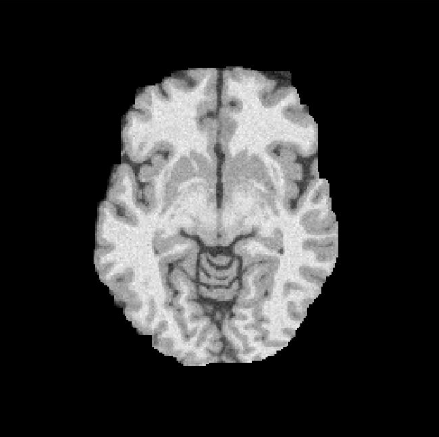
\includegraphics[width=\linewidth]{figures/Module_09/m09_5}
	\end{subfigure}
		\begin{subfigure}[b]{0.25\linewidth}
		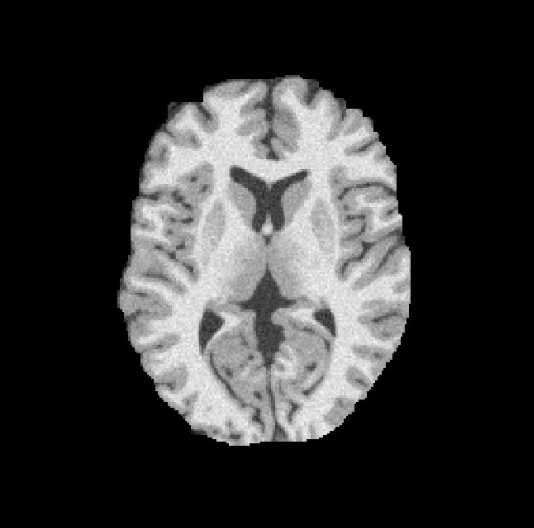
\includegraphics[width=\linewidth]{figures/Module_09/m09_6}
	\end{subfigure}
	\begin{subfigure}[b]{0.25\linewidth}
		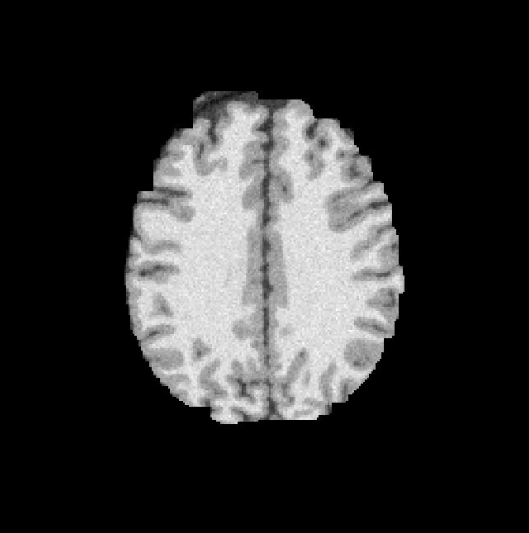
\includegraphics[width=\linewidth]{figures/Module_09/m09_7}
	\end{subfigure}
	\caption{Example of input data} 
	\label{fig:figures/m09_567}
\end{figure} 

An output data is NxM segmentation mask of image witheout nonbarin tissues (\ref{fig:figures/m09_1678}). 

\begin{figure}[H]
	\centering
	\begin{subfigure}[b]{0.25\linewidth}
		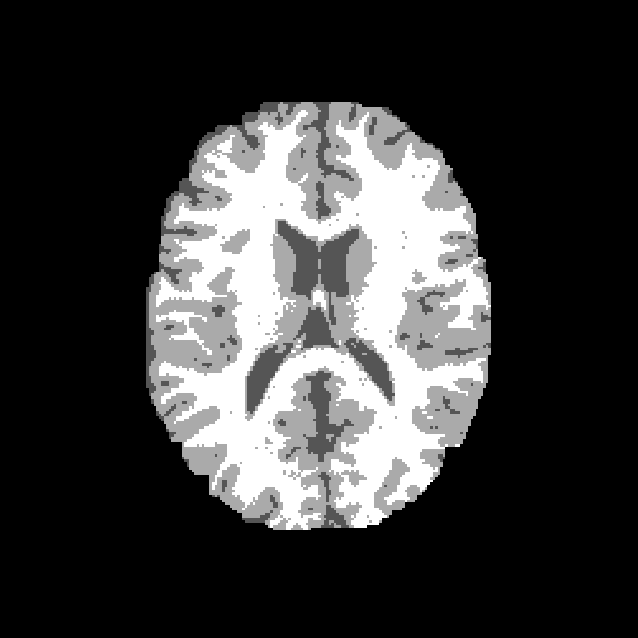
\includegraphics[width=\linewidth]{figures/Module_09/m09_16}
	\end{subfigure}
		\begin{subfigure}[b]{0.25\linewidth}
		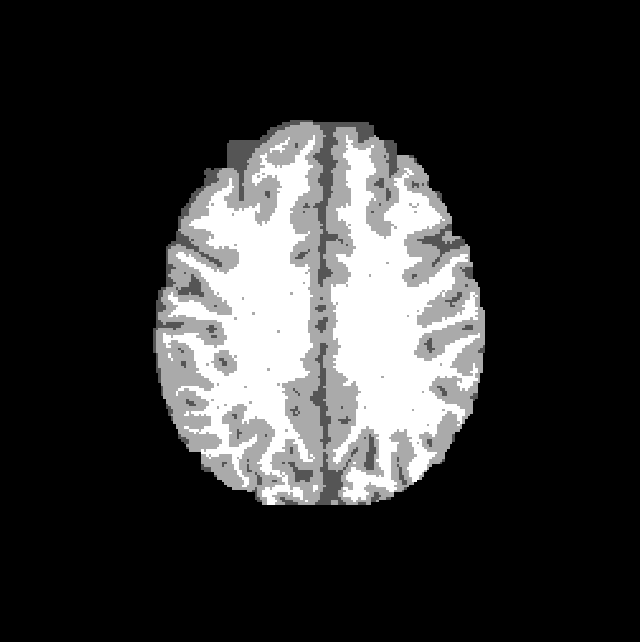
\includegraphics[width=\linewidth]{figures/Module_09/m09_17}
	\end{subfigure}
	\begin{subfigure}[b]{0.25\linewidth}
		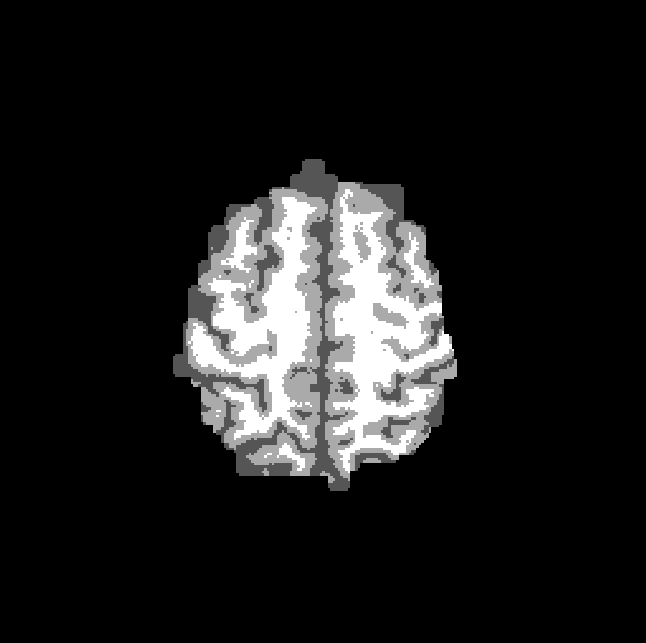
\includegraphics[width=\linewidth]{figures/Module_09/m09_18}
	\end{subfigure}
	\caption{Example of output data - segmentation masks} 
	\label{fig:figures/m09_1678}
\end{figure} 

\textbf{\textit{Libraries}}
In module, the basic python libraries are used:
\begin{itemize}
	\item math
	\item scipy 
	\item numpy
\end{itemize}

\textbf{\textit{Implementation}}
This module is used to brain MRI segmentation based on skull stripping images from Module 8. It consists of four functions:
\begin{itemize}
	\item imHist (image),
	\item imPart (skullFreeImage, firstPitch, lastPitch, rows, columns, pitches)
	\item gmm (x,mu,v,p),
	\item segmentation (skullFreeImage).
\end{itemize}

\textit{imHist function}
It is a function used for create image histogram. An image histogram is a chart that shows the distribution of intensities in an indexed or grayscale image. This is the first step of segmentation in every single slice of brain MRI image. In the beginning, to calculate the total number of image pixels, an array of image value is changing to vector. Next, by iterating by vector length, histogram is creating step by step (Fig. \ref{fig:figures/m09_11}). 
30/5000
The function argument is the \textbf{NxM single image}

\begin{figure}[H]
	\centering{}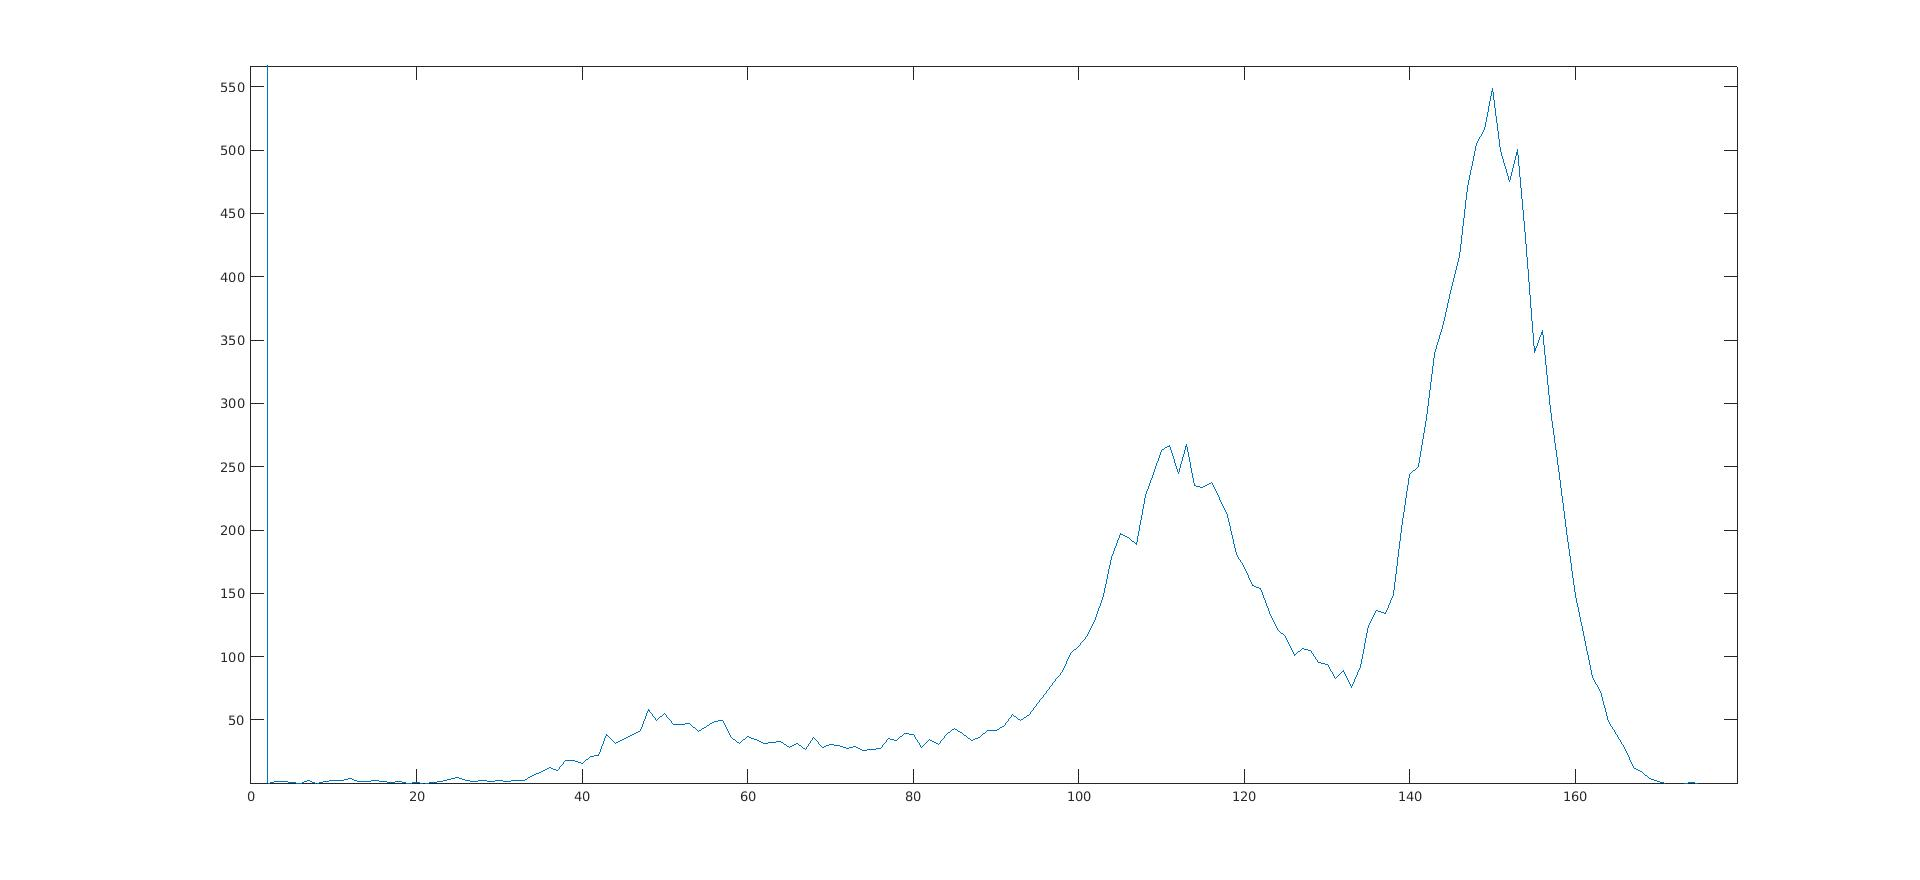
\includegraphics[width=0.7\textwidth]{figures/Module_09/m09_11}
	\caption{Image histogram  
	\label{fig:figures/m09_11}}
\end{figure} 

\begin{lstlisting}[language=Python, caption = Create image histogram]
for i in range(lengthImage):									# create histogram of non-zero image values
    f = int(floor(image[i]))									# round floor
    if f>0:
        if f<maxValue:
            odds=image[i]-f             						# difference between image and round floor image value
            a1=1-odds
            imageHistogram[f-1]=imageHistogram[f-1]+a1
            imageHistogram[f]=imageHistogram[f]+odds
            ...
            imageHistogram=np.convolve(imageHistogram,[1,2,3,2,1])# smoothing the histogram
\end{lstlisting}

At the end, histogram is smoothing by convolution with window [1,2,3,2,1] and noramlize by the sum of histogram values (\ref{fig:figures/m09_12}).

\begin{figure}[H]
	\centering{}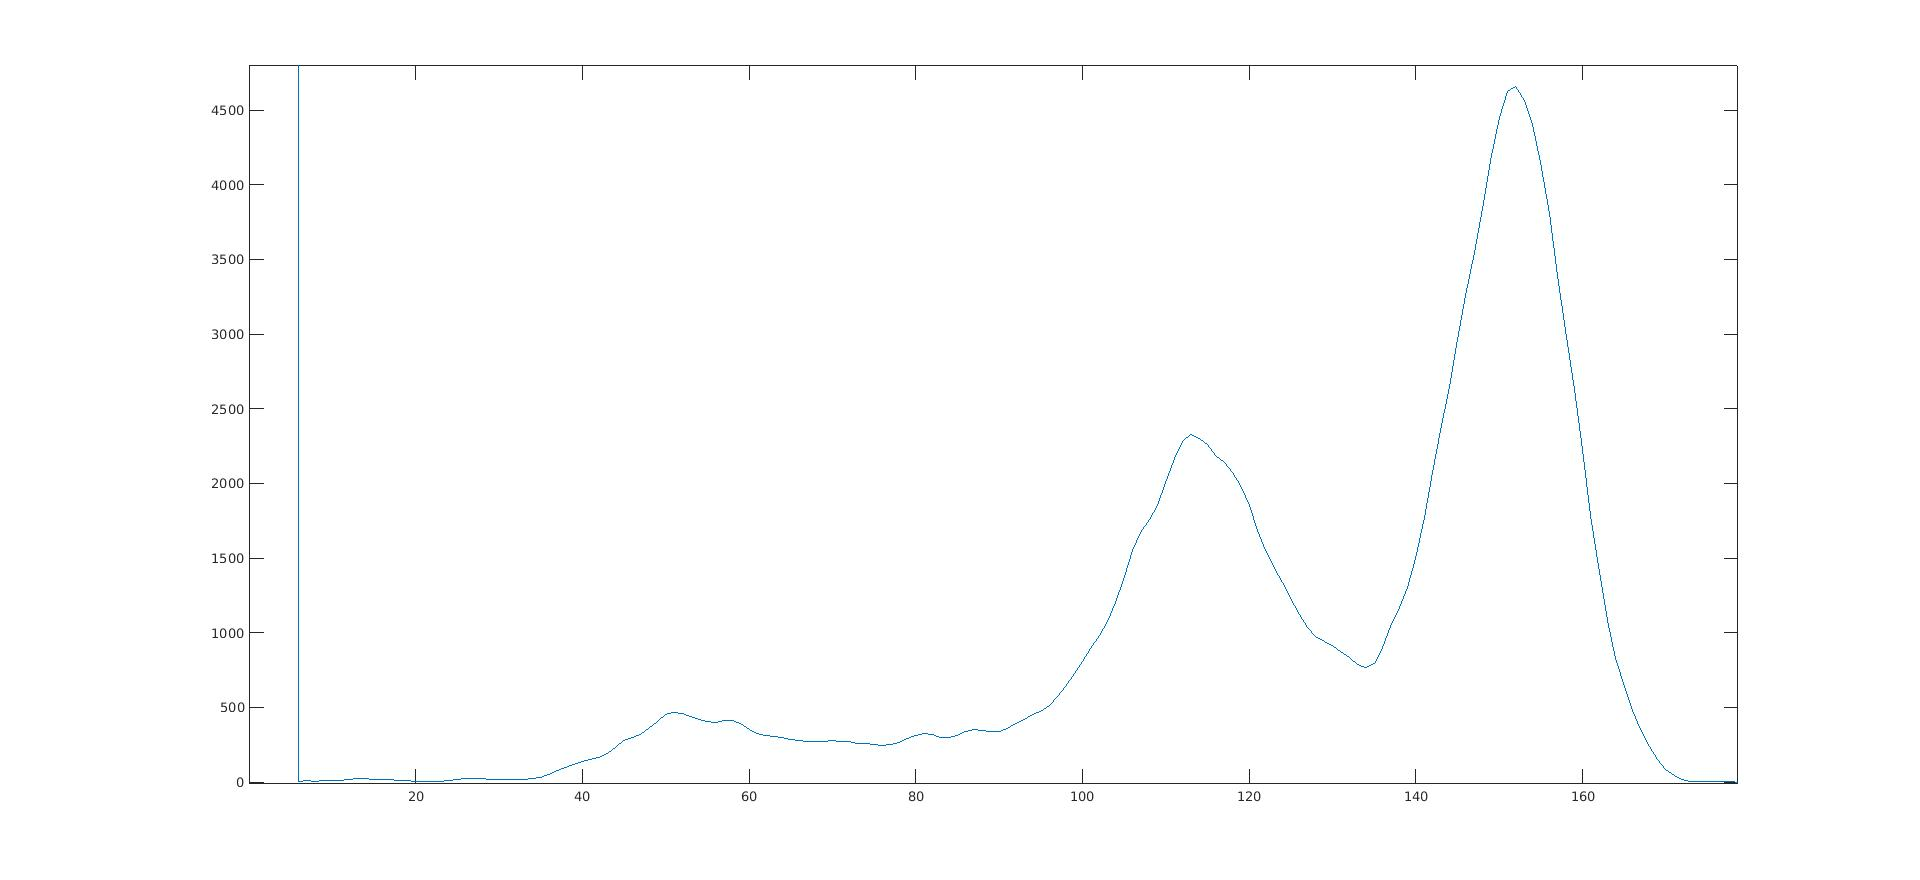
\includegraphics[width=0.7\textwidth]{figures/Module_09/m09_12}
	\caption{Image histogram  after smoothing by convolution
	\label{fig:figures/m09_12}}
\end{figure} 

\textit{imPart function}
It is a small function to get only image slices, which dosn't contain nonbrain tissues. In ths case, funtion gets 70 slices, from 70 to 140. Geting greater amonut can make issues. 
The function argument are: \textbf{image after skull stripping, number of first geting slice, number of last geting slice, image rows, image columns, number of slices}

\begin{lstlisting}[language=Python, caption = Geting part of image to segmentation]
for pitch in range (pitches):
    if pitch < firstPitch:
        continue
    if pitch >= firstPitch:
        if pitch < lastPitch:
            mageToSeg [:,:,rPit] = skullFreeImage [:,:,pitch]
            rPit = rPit+1
        else:
            break
\end{lstlisting}

\textit{gmm function}
The gmm function calculate mixture model gaussian distribution and and probability for each cluster of image data, based on mixture model initialize parameters
The function argument are: \textbf{x - histogram values vestor, mu - expectation values vector, v - variance vector, p - probability}

\begin{lstlisting}[language=Python, caption = gmm function]
for i in range(mu.size):
    differ=x-mu[i]
    mplitude = p[i]/(math.sqrt(2*math.pi*v[i]))
    app = amplitude*(np.exp((-0.5*(differ*differ))/v[i]))
    probab[:,i] = app	
\end{lstlisting}

\textit{segmentation function}
The segmentation function is the most important function in this module. It's utomatic algorithm, matching the Gaussian mixture model to the image histogram, in order to group pixels into proper cluster. To achieve the match, the expectation-maximization algorithm is used. 

The first step is inicialize Gaussian mixture model parameters vectors. They need to have the same numbers of element as numer of clusters. The initial parameters are choosen arbitrarily. It is important, to set different expected values to provide various algorithm starting points. 

\begin{lstlisting}[language=Python, caption = Segmentation -  parameters inicialization]
# alghoritm parameters inicialization 

clustersNum = 4					# number of clusters
mu = arange(1,clustersNum+1)*imMax/(clustersNum+1)	# expected value of each clusters
v = np.ones(clustersNum)*imMax		# variation of each clusters
p = np.ones(clustersNum)/clustersNum	# probability of each clusters
\end{lstlisting}

After inicialization, the algorithm starts its operation. It consists of two steps. The first one - expectation (step E) - use gmm function to deremine the gaussian distribution and check relative density using inicialized (in the first time) or updated distribution parameters. It calculate also the log-likelihood based on histogram values. 

\begin{lstlisting}[language=Python, caption = Segmentation - step E]
#Expectation Step

probab = gmm(x,mu,v,p)							# use gmm function - get probability
distrDens = probab.sum(axis=1)					# relative density 
llh = (hx*np.log(distrDens)).sum()				# the log-likelihood base on histogram data
\end{lstlisting}
The second step - maximization (step M) -  in which the model parameters are restimated using the distribution from step E

\begin{lstlisting}[language=Python, caption = Segmentation - step M]
#Maximization Step

for j in range(clustersNum):
    hxsh = hx.shape
    probabxh = probab.shape
    distsh=distrDens.shape
    resp = hx*probab[:,j]/distrDens			# compute the responsibilities
    p[j]=resp.sum()
    mu[j]=(x*resp/p[j]).sum()					# compute the weighted of expected values
    differ=x-mu[j]
    v[j]=(differ*differ*resp/p[j]).sum()		# compute the weighted varainces	
\end{lstlisting}

The algorithm's operation is shown below 

\begin{figure}[H]
	\centering{}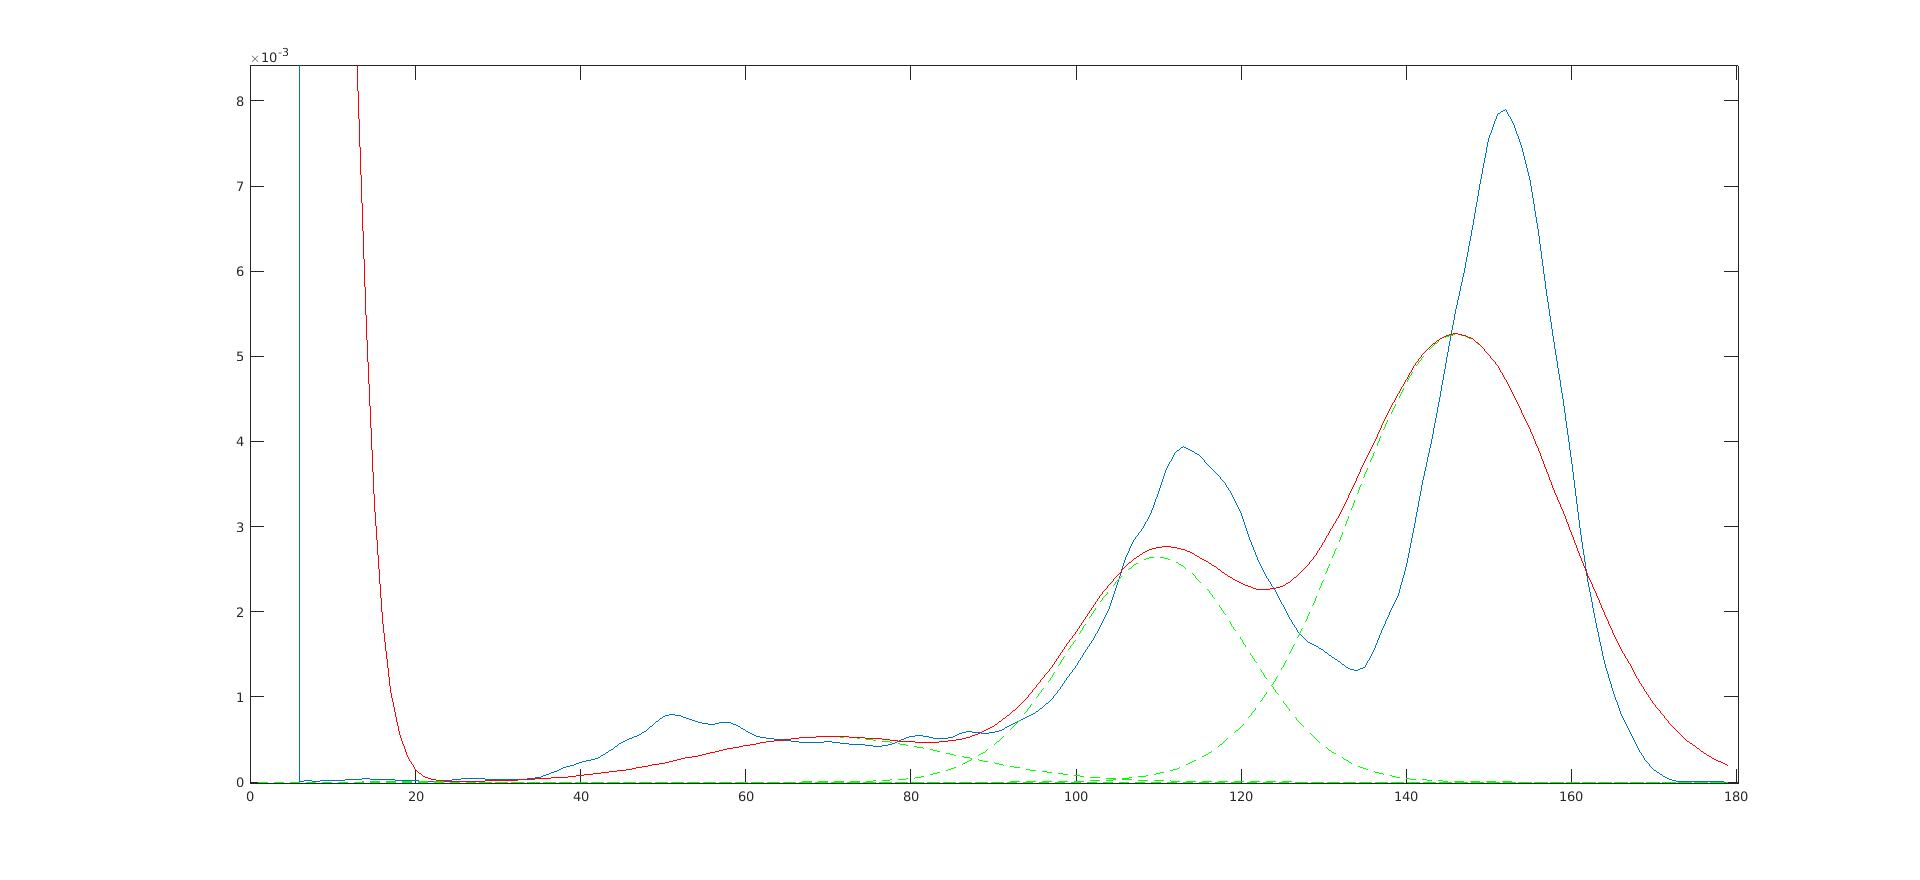
\includegraphics[width=0.7\textwidth]{figures/Module_09/m09_13}
	\caption{The first step - Gaussian mixture model after parameters inicialization
	\label{fig:figures/m09_13}}
\end{figure} 

\begin{figure}[H]
	\centering{}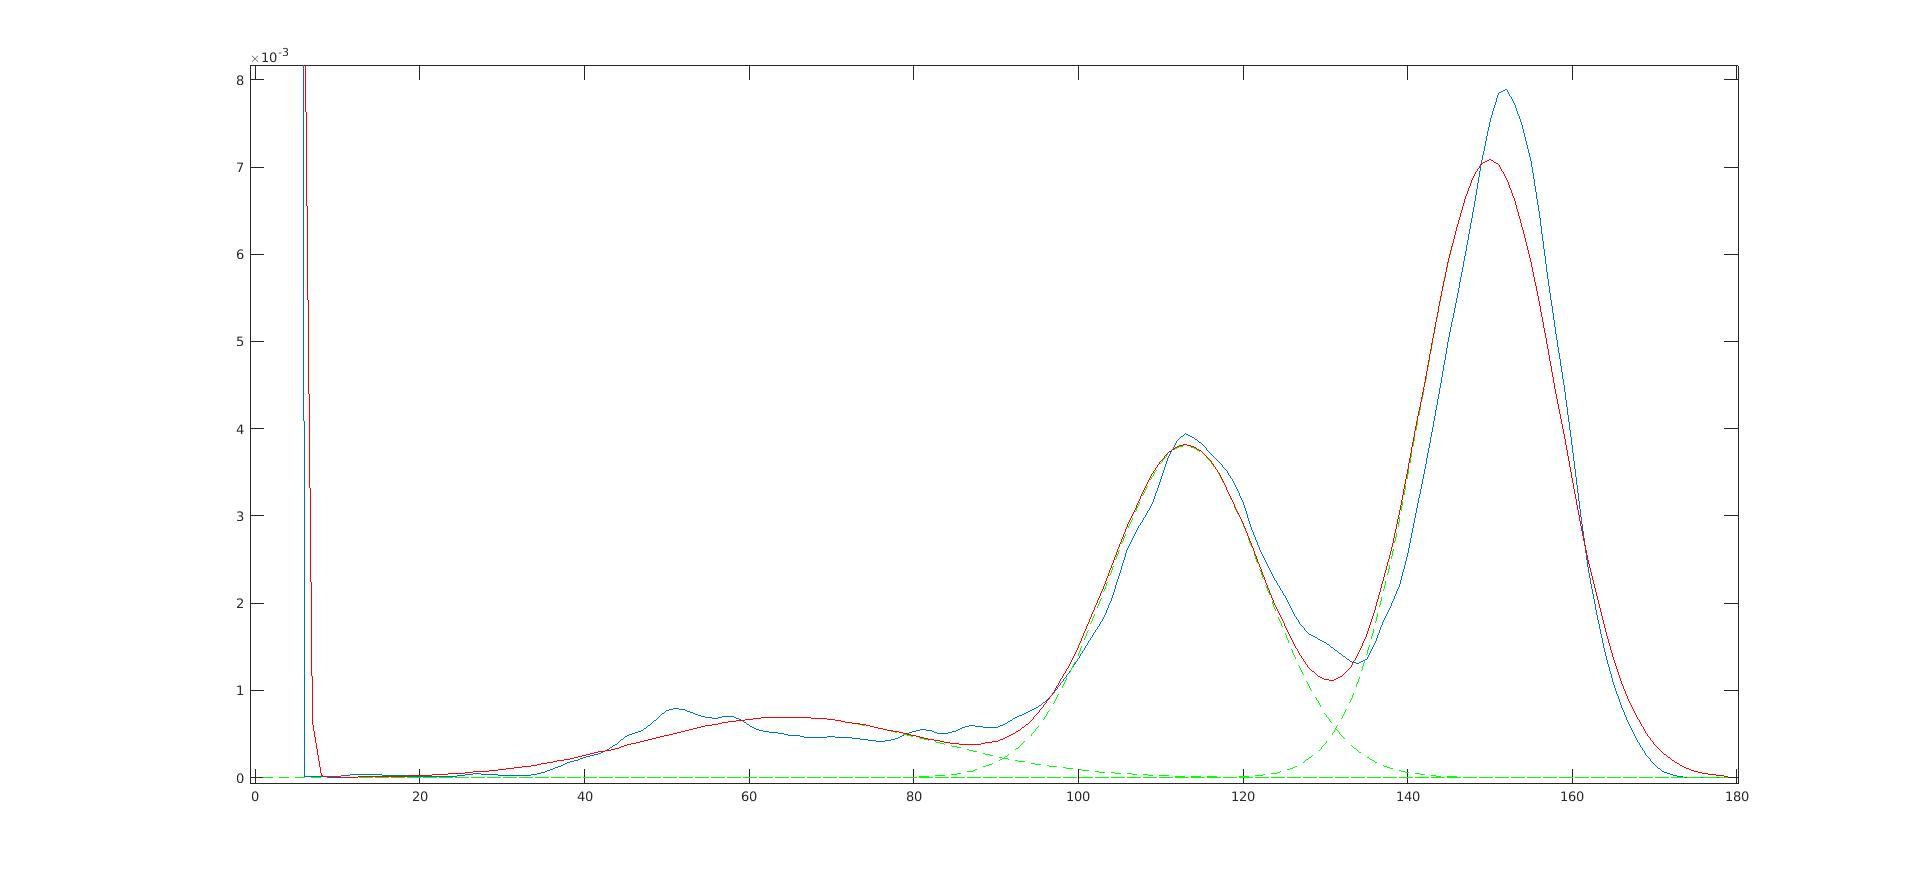
\includegraphics[width=0.7\textwidth]{figures/Module_09/m09_14}
	\caption{After few iteration - fitting Gaussian mixture model
	\label{fig:figures/m09_14}}
\end{figure} 

\begin{figure}[H]
	\centering{}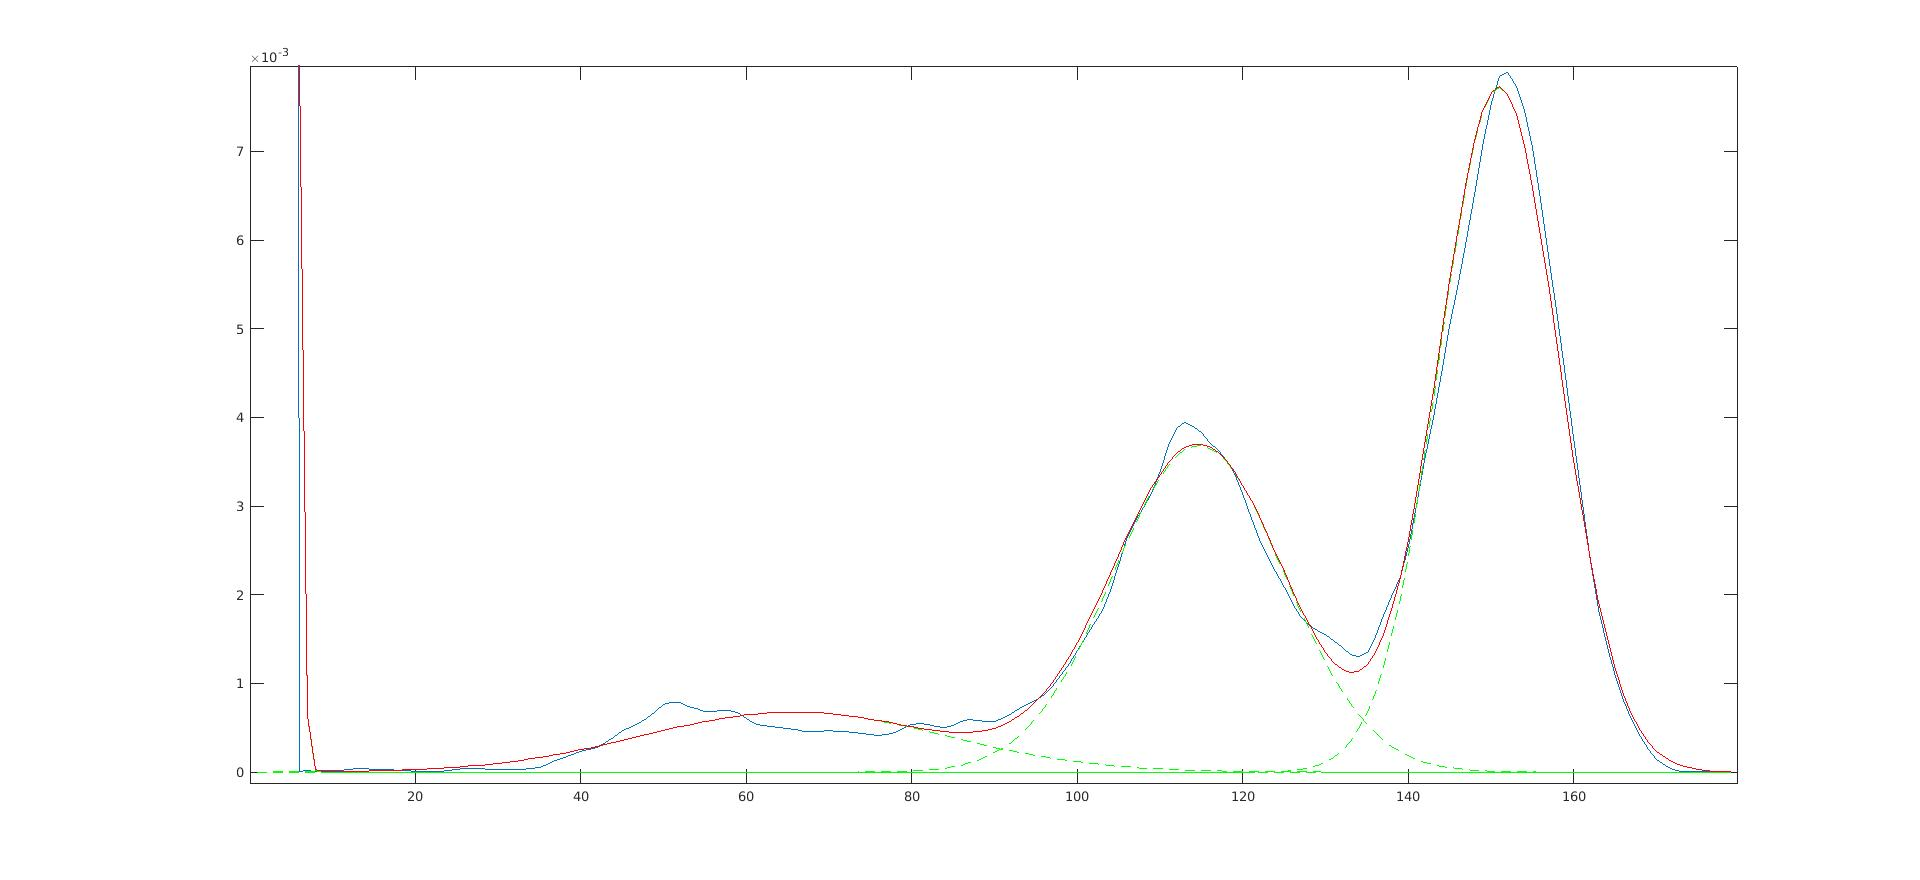
\includegraphics[width=0.7\textwidth]{figures/Module_09/m09_15}
	\caption{Result of matching  
	\label{fig:figures/m09_15}}
\end{figure} 

The last part of segmentation functiom is part, which creates image maske after segmenation (). Mask can be divided into 3 separated binary mask, represent white matter, gray matter and cerebrospinal fluid (Fig. \ref{fig:figures/m09_8910}).

\begin{lstlisting}[language=Python, caption = Create image mask]
# Creat image mask        
for i in range(rows):
	for j in range(columns):
    	for k in range(clustersNum):
        	c[k] = gmm(image[i,j],mu[k],v[k],p[k])
        a = (c==c.max()).nonzero()
        imageMask[i,j]=a[0]
\end{lstlisting}

\begin{figure}[H]
	\centering
	\begin{subfigure}[b]{0.25\linewidth}
		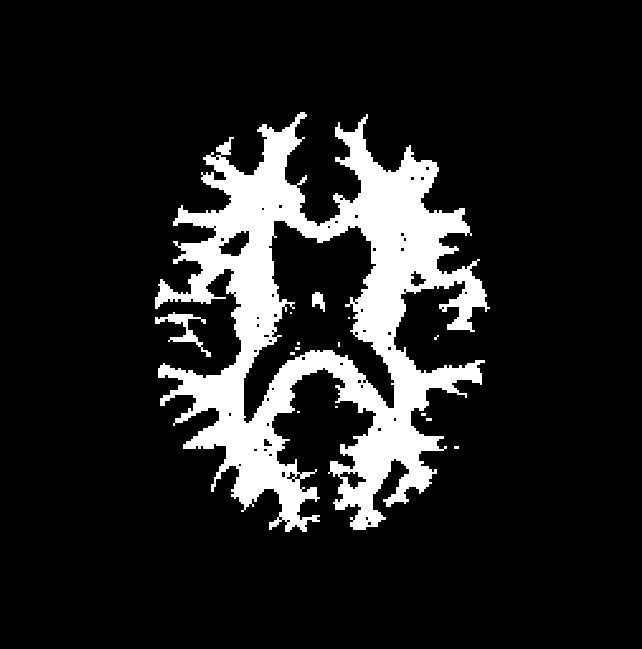
\includegraphics[width=\linewidth]{figures/Module_09/m09_8}
		\caption{a}
	\end{subfigure}
		\begin{subfigure}[b]{0.25\linewidth}
		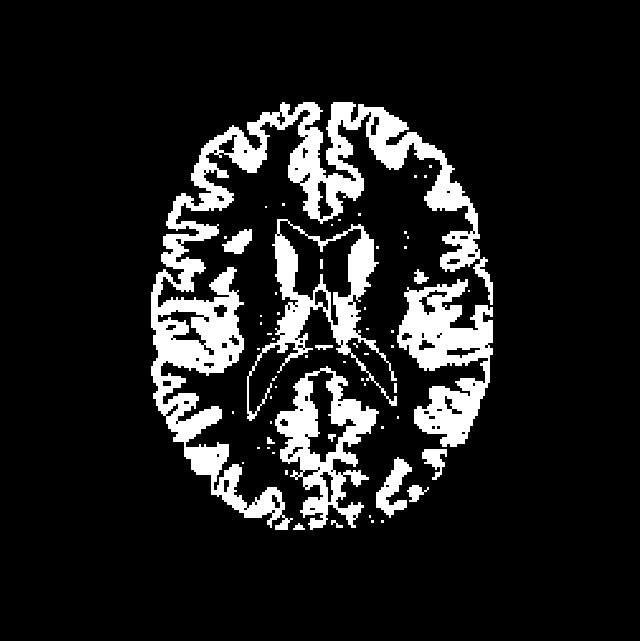
\includegraphics[width=\linewidth]{figures/Module_09/m09_10}
		\caption{b}
	\end{subfigure}
	\begin{subfigure}[b]{0.25\linewidth}
		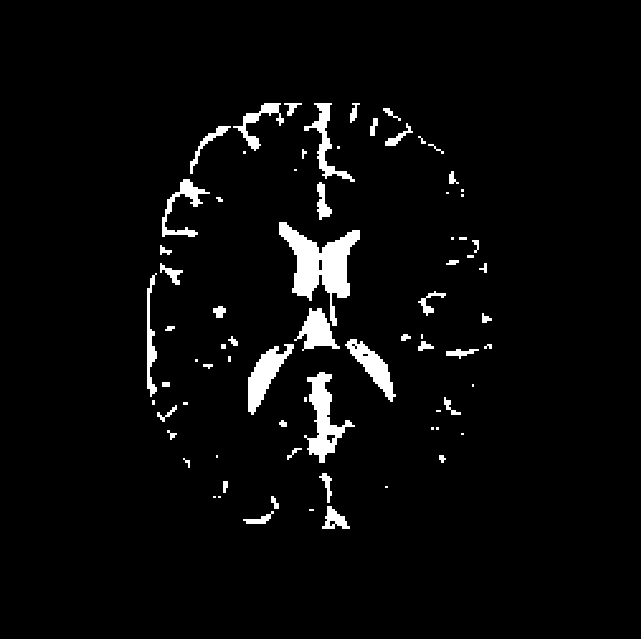
\includegraphics[width=\linewidth]{figures/Module_09/m09_9}
		\caption{c}
	\end{subfigure}
	\caption{Isolated barin structure: a) white matter, b) gray matter, c) cerebrospinal fluid} 
	\label{fig:figures/m09_8910}
\end{figure} 